\subsection{Graphics Processing Units, accessible high performance parallel computing}
\label{sec:gpu}

In the development of microprocessors, the addition of new cores is now the
way forward, rather than the improvement of single thread performance.
Graphics processing units (GPUs) have moved from being specialised graphics
engines to being suitable to tackle applications with high computational
demands. For a recent survey of the hardware, programming methods and tools,
and successful applications, the reader is referred to~\citeifl{GPUComputing}.
Figure~\ref{fig:image}, taken from that paper, and due to NVIDIA, shows the
architecture of a modern GPU from NVIDIA. It contains 16 multiprocessors, 
grouped in pairs that share a texture fetch unit (TF in the figure). The 
texture fetch unit is of little importance when using the GPU for general 
purpose computations. Each multiprocessor has 8 stream processors (marked 
SP in the figure). These stream processors has access to 16kB of shared memory.  

See reference~\citeifl{GPUComputing} for information about
the very similar AMD GPU architecture. We have used the NVIDIA architecture,
but developments are similar at AMD. Intel's Larrabee processor points to a
future in which each individual core is considerably more powerful than in
today's GPUs~\citeifl{larrabee}.

%along with shared data and instruction caches, and 16kB of shared memory. 

The question of how to program powerful data-parallel processors is likely
to continue to be an interesting one. Unlike for current multicore machines,
the question here is how to keep a large number of small processors
productively occupied. NVIDIA's solution has been to develop the
architecture and the programming model in parallel. The result is called
CUDA -- an extension of C designed to allow developers to exploit the power
of GPUs. Reference~\citeifl{GPUCudaLuebke} gives a very brief but illuminating
introduction to CUDA for potential new users. The idea is that the user
writes small blocks of straightforward C code, which should then run in
thousands or millions of threads. We borrow the example from the above
introduction. To add two $N \times N$ matrices on a CPU, using C, one would
write something like

\begin{code}
// add 2 matrices on the CPU:
void addMatrix(float *a, float *b, float *c, int N)
{
  int i, j, index;
  for (i = 0; i < N; i++) {
    for (j = 0; j < N; j++) {
      index = i + j * N;
      c[index]=a[index] + b[index];
    }
  }
}
\end{code}
\FloatBarrier

\begin{figure}%
\begin{center}
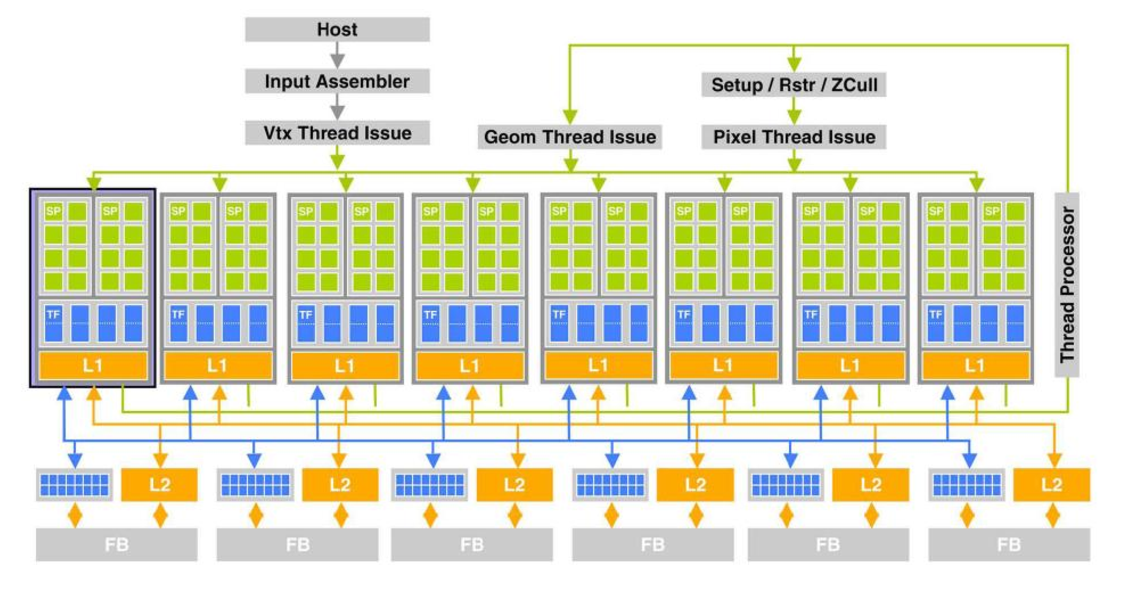
\includegraphics[height = 6cm]{./ifl/image_top.pdf}
%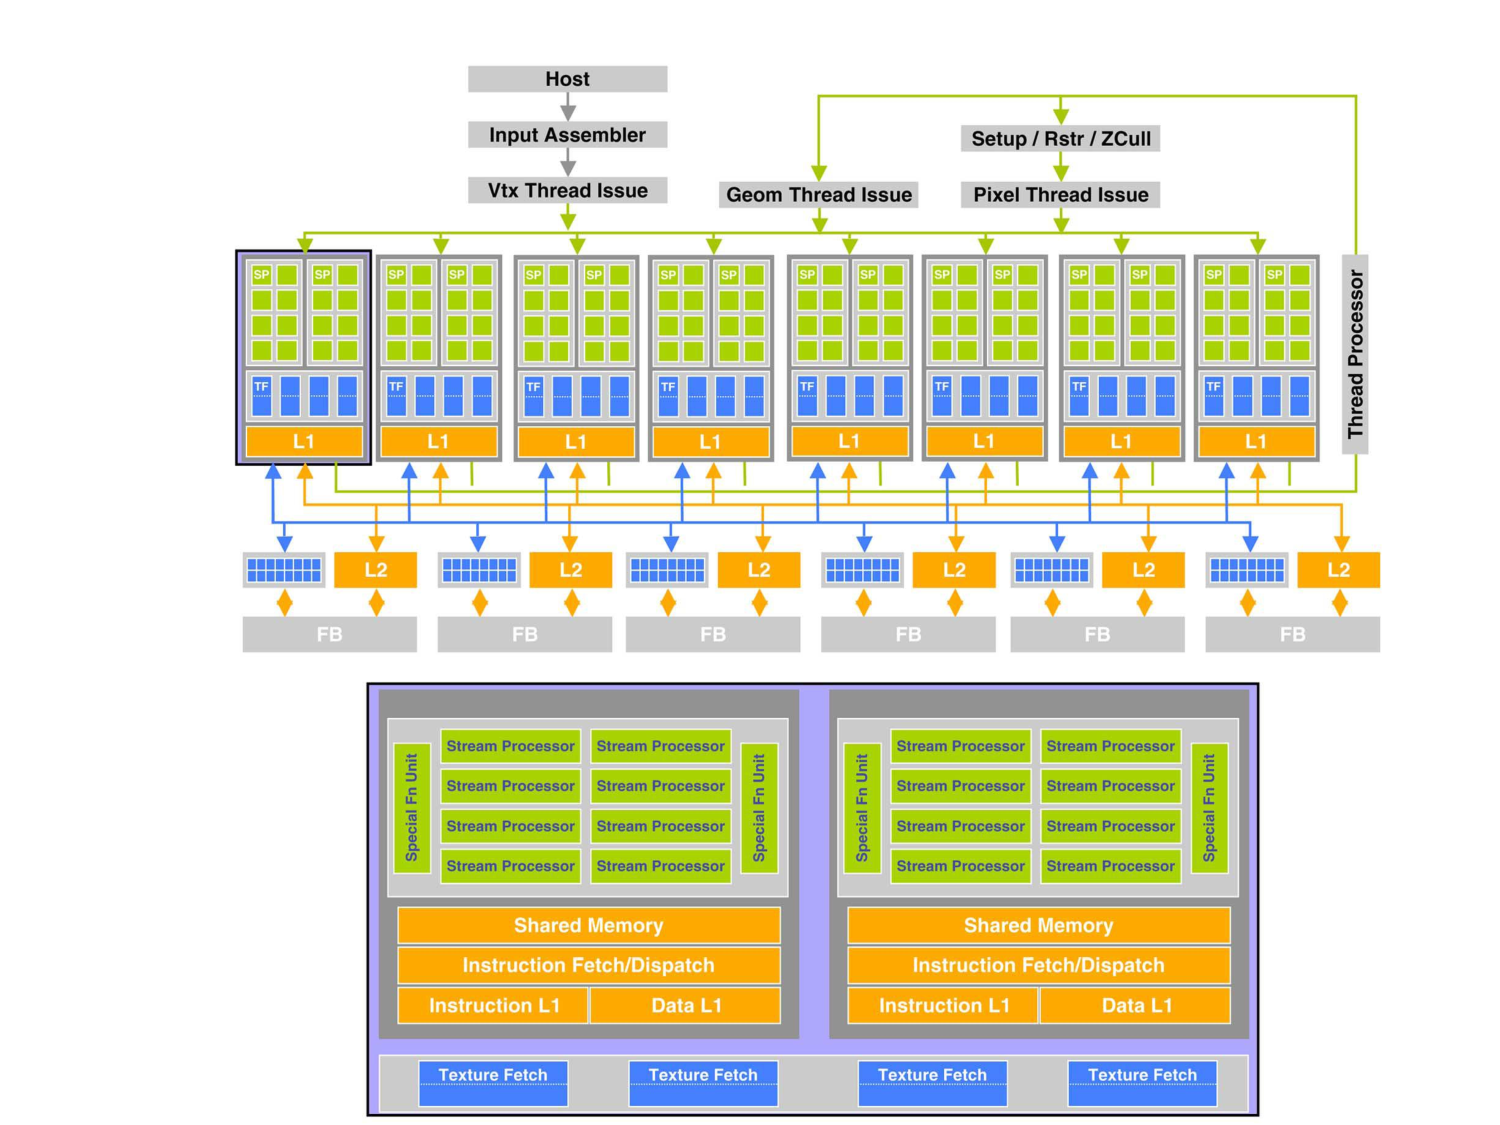
\includegraphics[width = 14cm]{image.pdf}
\caption{The NVIDIA 8800GTX GPU architecture, with 8 pairs of multiprocessors. Diagram courtesy of NVIDIA.}\label{fig:image}
\end{center}
\end{figure}


\noindent In CUDA, one writes a similar C function, called a {\em kernel},
to compute one element of the matrix. Then, the kernel is invoked as many
times as the matrix has elements, resulting in many threads, which can be
run in parallel. A predefined structure called {\tt threadIdx} is used to
label each of these many threads, and can be referred to in the kernel.
\begin{code}
// add 2 matrices on the GPU (simplified)
__global__ void addMatrix(float *a,float *b, float *c, int N)
{
  int i= threadIdx.x;
  int j= threadIdx.y;
  int index= i + j * N;
  c[index]= a[index] + b[index];
}

void main()
{
  // run addMatrix in 1 block of NxN threads:
  dim3 blocksize(N, N),
  addMatrix<<<1, blocksize>>>(a, b, c, N);
}
\end{code}
Here, a two dimensional {\em thread block} of size $N \times N$ is created.

CUDA uses {\em barrier synchronisation} and {\em shared memory} for
introducing communication between threads. Contents of shared memory (16kB
per multiprocessor in the architecture shown in Figure~\ref{fig:image}) is
visible to all threads in a thread block. It is very much faster to access
this shared memory than to access the global device memory. We shall see
later that Obsidian provides users with both shared and global arrays,
giving the user control over where data is to be stored.

Since many threads are now writing and reading from the same shared memory,
it is necessary to have a mechanism that enables the necessary
synchronisation between threads. CUDA provides a barrier synchronisation
mechanism called {\tt \_\_syncthreads()}. Only when all threads in a block
have reached this barrier can any of them proceed. This allows the
programmer to ensure safe access to the shared memory for the many threads
in a thread block.

Now, a {\em grid} is a collection of thread blocks. Each thread block runs
on a single multiprocessor, and the CUDA system can schedule these individual
blocks in order to maximise the use of GPU resources. A complete program
then consists not only of the kernel definitions, but also of code, to be
run on the CPU, to launch a kernel on the GPU, examine the results and
possibly launch new kernels. In this paper, we will not go into details
about how kernels are coordinated, but will concentrate on how to write
individual kernels, as this is the part of Obsidian that is most developed.
In Obsidian, we write code that looks like the Lava descriptions in
section~\ref{sec:combinators}, and we generate CUDA code like that shown
above. This is a considerably more complex process than the generation of
netlists in Lava.


